% William, Nikhil, Eashan, Rishit, Sahil, Sarvesh

\documentclass{article}
\usepackage[english]{babel}
\usepackage[utf8]{inputenc}
\usepackage{amsmath}
\usepackage{amsfonts}
\usepackage{amssymb}
\usepackage{graphicx}
\usepackage{enumitem}
\usepackage{tikz}
\usepackage{float}
\usetikzlibrary{decorations.pathreplacing}
\usetikzlibrary{shapes.geometric}

\title{Graphene Rotational Acceleration\\Particle Hall Sensor (GRAPHS)}
\author{Nikhil Vijay, William Forte, Eashan Iyer,\\Rishit Arora, Sahil Shah, Sarvesh Patham}
\date{\today}

\begin{document}
    \maketitle

    \section{Why we want to come to CERN}
    \indent As students with a deep curiosity for modern physics, this competition gives us the freedom to pursue our own research and provides the possibility of visiting the facilities at CERN, a fascinating opportunity. Our experiment would be insightful for understanding graphene's properties by making an entirely mechanical particle detector, building off the ideas of solar sails. CERN is the only place that could make this possible with the cutting-edge facilities of the beamline: particle accelerators and advanced detectors would provide opportunities to study graphene in a highly-controlled environment. Additionally, CERN is incredible due to the experienced researchers operating there, whom we would be thrilled to learn from and collaborate with.

    \section{Experiment motivation}
    \indent It has been established that graphene is an optimal material for solar sails \cite{GAUDENZI} due to its acute response to photon-induced movement by radiation pressure. We were interested in investigating the use of this property to detect the presence of particles.

    \section{The experiment}

    \begin{figure}[H]
    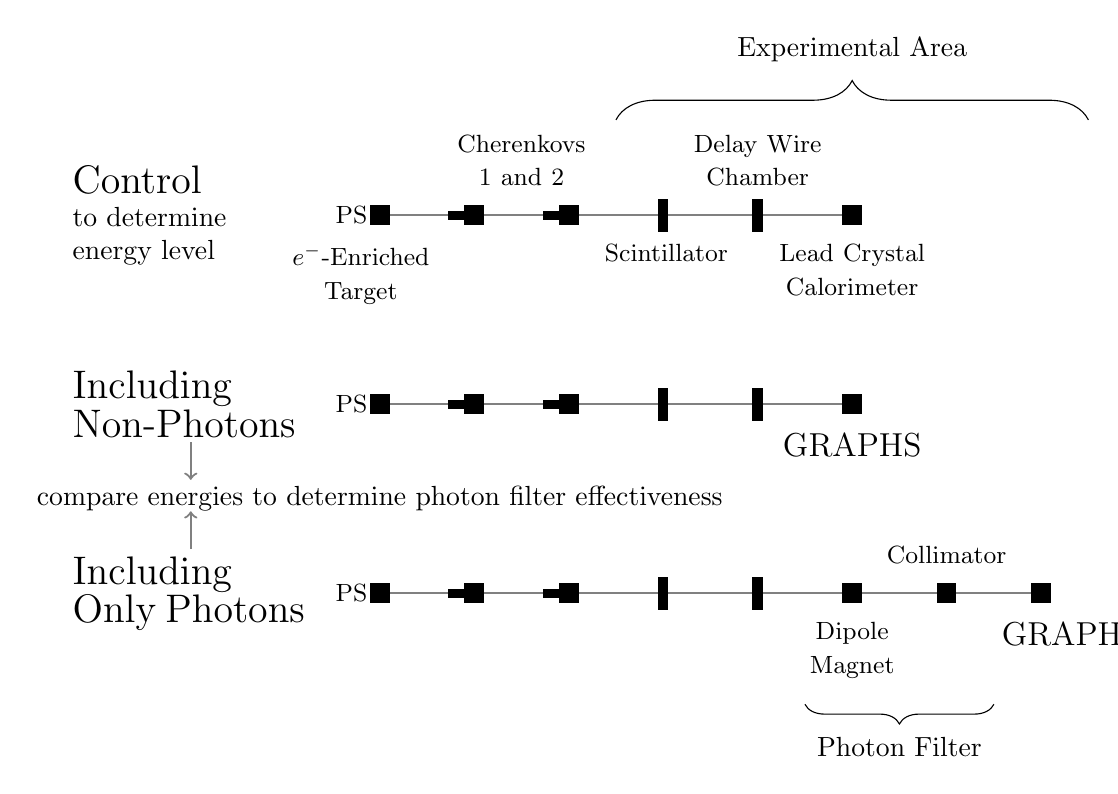
\begin{tikzpicture}[scale=0.8, xscale=1.5]
        \draw[decorate,decoration={brace, amplitude=0.5cm, raise=8ex}] (3.5,0) -- (8.5,0) node[midway, yshift=6em]{Experimental Area};
        \node[fill=white, text width=3cm] at (-1,0) {\Large{Control} \normalsize{\\to determine\\energy level}};
        \node[fill=white] at (0.7,0) {\small{PS}};
        \draw[gray, thick] (1,0) -- (2,0) -- (3,0) -- (4,0) -- (5,0) -- (6,0);
        \node[rectangle, draw, fill, black] at (1,0) {};
        \node[rectangle, draw, fill, black] at (2,0) {};
        \node[rectangle, draw, fill, black, inner ysep=0.05cm, inner xsep=0.2cm] at (1.9,0) {};
        \node[rectangle, draw, fill, black] at (3,0) {};
        \node[rectangle, draw, fill, black, inner ysep=0.05cm, inner xsep=0.2cm] at (2.9,0) {};
        \node[rectangle, draw, fill, black, inner ysep=0.2cm, inner xsep=0.06cm] at (4,0) {};
        \node[rectangle, draw, fill, black, inner ysep=0.2cm, inner xsep=0.06cm] at (5,0) {};
        \node[rectangle, draw, fill, black] at (6,0) {};
        \node[below=0.25cm, text width=2cm, align=center] at (0.8,0) {\small{$e^{-}$-Enriched Target}};
        \node[above=0.25cm, text width=2cm, align=center] at (2.5,0) {\small{Cherenkovs 1 and 2}};
        \node[below=0.25cm, text width=1cm, align=center] at (3.8,0) {\small{Scintillator}};
        \node[above=0.25cm, text width=2cm, align=center] at (5,0) {\small{Delay Wire Chamber}};
        \node[below=0.25cm, text width=2cm, align=center] at (6,0) {\small{Lead Crystal Calorimeter}};

        \node[text width=3cm] at (-1,-3) {\Large{Including Non-Photons}};
        \node[fill=white] at (0.7,-3) {\small{PS}};
        \draw[gray, thick] (1,-3) -- (2,-3) -- (3,-3) -- (4,-3) -- (5,-3) -- (6,-3);
        \node[rectangle, draw, fill, black] at (1,-3) {};
        \node[rectangle, draw, fill, black] at (2,-3) {};
        \node[rectangle, draw, fill, black, inner ysep=0.05cm, inner xsep=0.2cm] at (1.9,-3) {};
        \node[rectangle, draw, fill, black] at (3,-3) {};
        \node[rectangle, draw, fill, black, inner ysep=0.05cm, inner xsep=0.2cm] at (2.9,-3) {};
        \node[rectangle, draw, fill, black, inner ysep=0.2cm, inner xsep=0.06cm] at (4,-3) {};
        \node[rectangle, draw, fill, black, inner ysep=0.2cm, inner xsep=0.06cm] at (5,-3) {};
        \node[rectangle, draw, fill, black] at (6,-3) {};
        \node[below=0.25cm, text width=2cm, align=center] at (6,-3) {\large{GRAPHS}};

        \node[text width=3cm] at (-1,-6) {\Large{Including Only Photons}};
        \node[fill=white] at (0.7,-6) {\small{PS}};
        \draw[gray, thick] (1,-6) -- (2,-6) -- (3,-6) -- (4,-6) -- (5,-6) -- (6,-6) -- (7,-6) -- (8,-6);
        \node[rectangle, draw, fill, black] at (1,-6) {};
        \node[rectangle, draw, fill, black] at (2,-6) {};
        \node[rectangle, draw, fill, black, inner ysep=0.05cm, inner xsep=0.2cm] at (1.9,-6) {};
        \node[rectangle, draw, fill, black] at (3,-6) {};
        \node[rectangle, draw, fill, black, inner ysep=0.05cm, inner xsep=0.2cm] at (2.9,-6) {};
        \node[rectangle, draw, fill, black, inner ysep=0.2cm, inner xsep=0.06cm] at (4,-6) {};
        \node[rectangle, draw, fill, black, inner ysep=0.2cm, inner xsep=0.06cm] at (5,-6) {};
        \node[rectangle, draw, fill, black] at (6,-6) {};
        \node[rectangle, draw, fill, black] at (7,-6) {};
        \node[rectangle, draw, fill, black] at (8,-6) {};
        \node[below=0.25cm, text width=2cm, align=center] at (6,-6) {\small{Dipole Magnet}};
        \node[above=0.25cm, text width=2cm, align=center] at (7,-6) {\small{Collimator}};
        \node[below=0.25cm, text width=1cm, align=center] at (8,-6) {\large{GRAPHS}};

        \node[fill=white, align=right] at (1,-4.5) {\normalsize{compare energies to determine photon filter effectiveness}};
        \draw[gray, thick, ->] (-1,-3.6) -- (-1, -4.2);
        \draw[gray, thick, ->] (-1,-5.3) -- (-1, -4.7);

        \draw[decorate,decoration={brace, amplitude=0.25cm, mirror, raise=8ex}] (5.5,-6.25) -- (7.5,-6.25) node[midway, yshift=-5em]{Photon Filter};
    \end{tikzpicture}
    \caption{T9 beam diagrams for various tests.}
    \end{figure}

\indent Our experiment seeks to determine the effect of particle collisions on graphene, both by photons (as in solar sails) and other particles.

	Using the calorimeter as a control, we are able to establish the particle energy to be absorbed by the graphene in our second test, allowing us to determine the efficiency of the energy's conversion into rotational energy.

    \indent To establish a beam of photons (photon filter in fig. 1), a dipole magnet (or a substitute) can filter charged particles\cite{BEAM2018}, causing a small angular divergence by a large Lorentz factor\cite{OHKUMA}. Charged particles can then be filtered through a collimator.

    The impact of non-photons is unclear since the half-life of pions is short and muons from pion decay pass through meters of iron with little stopping power as in CERN's muon filters\cite{BEAM2018}, whereas the stopping power of photons is initially high \cite{SABIN}. This is why there are two GRAPHS tests--one with photon filtering and one without--to assess the impact of non-photons, detected as a difference in data between them.

    \subsection{Experimental conditions}

    \indent In order to eliminate as many external factors as possible, the experiment would occur in a vacuum and the apparatus would be inside a vibration-isolating environment.

    \subsection{Detector construction}

\indent The detector is made of a rectangular monolayer of graphene, approximately 1mm by 0.5mm. This sheet would be held in a 40 gauge titanium wire frame to add flex resistance with little inertia due to low density. On the top of the graphene, the titanium wire is attached to a neodymium magnet. This magnet would be levitated under a type II superconductor, locking the magnet from moving along its x and y-axis (fig. 2) and facilitating rotation with minimal resistance. A high-gauge paramagnetic wire (magnetized by the neodymium magnet) will be attached from the neodymium magnet, down the titanium wire and below the graphene. A hall effect sensor will be placed below the magnetic wire to detect changes in the magnetic field as the graphene and the magnetic wire rotate.

    \begin{figure}[H]
    \begin{tikzpicture}[scale=1]
        \draw[gray,thick, <-] (0,0.2) -- (2.4,1.3);
        \draw[gray,thick, ->] (2.4,1.3) -- (4.8, 0.2);
        \draw[gray,thick, ->] (2.4,1.3) -- (2.4,6);
        \draw[gray,thick] (8,1.6) -- (3.5,3.6) -- (3.5,6.5) -- (8,4.5) -- (8,1.6);

        \draw[gray,thick] (8.1,1.56) -- (3.4,3.64) -- (3.4,6.7) -- (8.1,4.6) -- (8.1,1.56);
        \node[above=0.25cm, align=center] at (6.2, 6.4) {\normalsize{titanium brace}};
        \draw[gray,thick,dashed] (6.2,6.65) -- (5.5,5.8);

        \draw[gray,thick] (8.2,0.9) -- (6.0,1.8) -- (6.0, 2.35);
        \draw[gray,thick] (6.0,2.34) -- (8.2,1.36);
        %\node[align=center] at (6.5, 1.8) {\normalsize{N}};
        %\node[align=center] at (7.7, 1.3) {\normalsize{S}};
        \draw[<-] (8.1, 2.4)  to [out=-45,in=-30, looseness=2] (8.6,2.6);

        \draw[gray,thick] (8.2,1.35) -- (8.2, 4.4);
        \draw[gray,thick] (8.4,0.8) -- (8.4, 4.3);
        \draw[gray,thick] (8.2, 4.4) -- (8.4, 4.3);
        \draw[gray,thick] (8.2,0.9) -- (8.4, 0.8);

        \draw[gray,thick] (8.2,4.4) -- (8.3, 4.5);
        \draw[gray,thick] (8.5,0.9) -- (8.5, 4.4);
        \draw[gray,thick] (8.3, 4.5) -- (8.5, 4.4);
        \draw[gray,thick] (8.5,0.9) -- (8.4,0.8);
        \draw[gray,thick] (8.5,4.4) -- (8.4,4.3);
        \draw[gray,thick,dashed] (8.35, 4.8) -- (8.35, 5.4);

        \draw[gray,thick, ->] (2,2.6) -- (5.6,4.1);
        \draw[<-] (8.1, 4.1)  to [out=-45,in=0, looseness=3] (8.3,4.6);
        \node[above=0.4cm, text width=2cm, align=center] at (5.0,3.6) {\normalsize$particles$};
        \node[above=0.25cm, text width=2cm, align=center] at (2.4,6) {\LARGE$y$};
        \node[above=0.25cm, text width=2cm, align=center] at (4.8,0.2) {\LARGE$x$};
        \node[above=0.25cm, text width=2cm, align=center] at (0,0.2) {\LARGE$z$};
        \node[align=center,rotate=-23.5] at (5.5, 5.3) {\small{graphene monolayer}};

        \node[ellipse,draw, minimum width=1cm, minimum height=0.75cm] at (8.35,6.8) {};
        \draw (7.85,6.0) arc(180:360:0.5cm and 0.375cm);
        \draw (7.85,6.4) arc(180:360:0.5cm and 0.375cm);
        \draw[gray,thick] (7.85,6.0) -- (7.85,6.8);
        \draw[gray,thick] (8.85,6.0) -- (8.85,6.8);

        \node[ellipse,draw, minimum width=1cm, minimum height=0.75cm] at (8.35,8.8) {};
        \draw (7.85,8.0) arc(180:360:0.5cm and 0.375cm);
        \draw[gray,thick] (7.85,8.0) -- (7.85,8.8);
        \draw[gray,thick] (8.85,8.0) -- (8.85,8.8);
        \draw[gray,thick,dashed] (8.35, 7.25) -- (8.35, 7.6);
        \draw[decorate,decoration={brace, amplitude=0.25cm, raise=6ex}] (8.2,7.5) -- (8.2,9.25) node[midway, xshift=-7.5em]{superconductor};

        \draw[gray,thick] (6.0,-0.4) -- (5.5,-0.2) -- (5.5,0.4) -- (6.0, 0.2) -- (6.0, -0.4);
        \draw[gray,thick] (6.7,0.9) -- (7.2, 0.7) -- (7.2,0.1);
        \draw[gray,thick] (5.5,0.4) -- (6.7,0.9);
        \draw[gray,thick] (6.0,-0.4) -- (7.2,0.1);
        \draw[gray,thick] (6.0,0.2) -- (7.2,0.7);
        \node[align=center] at (6.5, 0.1) {\small{Hall}};
        \node[align=center] at (8.4, 6.2) {\small{N}};
        \node[align=center] at (8.4, 5.8) {\small{S}};
        \draw[decorate,decoration={brace, amplitude=0.25cm, mirror, raise=8ex}] (7.5,0.4) -- (7.5,3.0) node[midway, xshift=9.5em]{paramagnetic wire};

        \node[opacity=0.15] at (5.65,4.0) {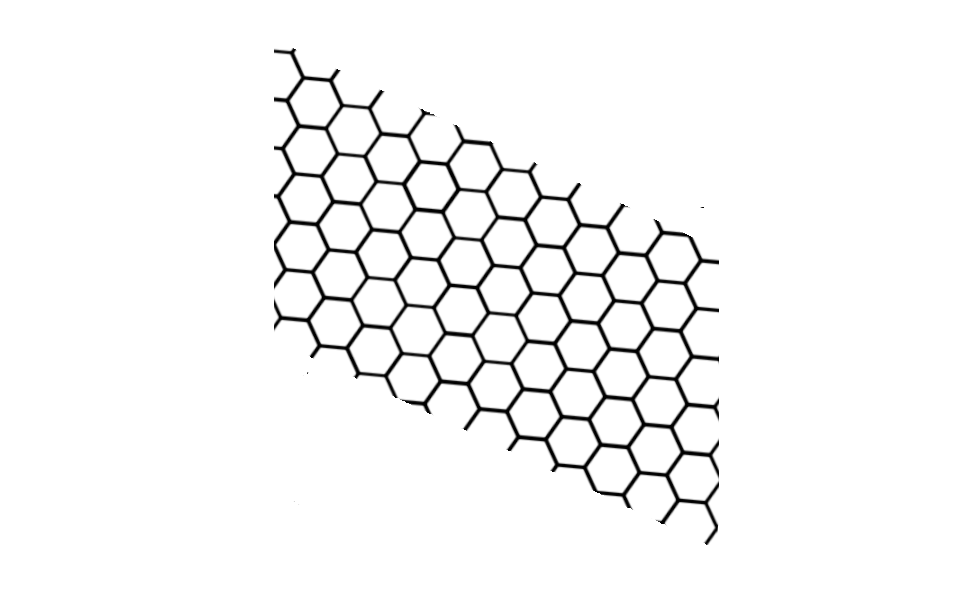
\includegraphics[width=9.5cm,height=5.65cm]{hex_lattice_perspective.png}};
    \end{tikzpicture}
    \caption{The structure of GRAPHS}
    \end{figure}

After the energy of the particles has been established through the control calorimeter test, another beam of similar energy is shot at the center of the graphene for a time, t. With a certain efficiency, some of the particle's momentum is going to be transferred to the graphene, causing an angular acceleration about the y-axis. As the graphene rotates, so does the bottom magnetic wire, causing a change in magnetic flux detectable by the hall effect sensor. Using sensor data, we can find out the angular acceleration of the graphene to figure out the percentage of momentum that was transferred to the graphene from the particle.

    \begin{figure}[H]
    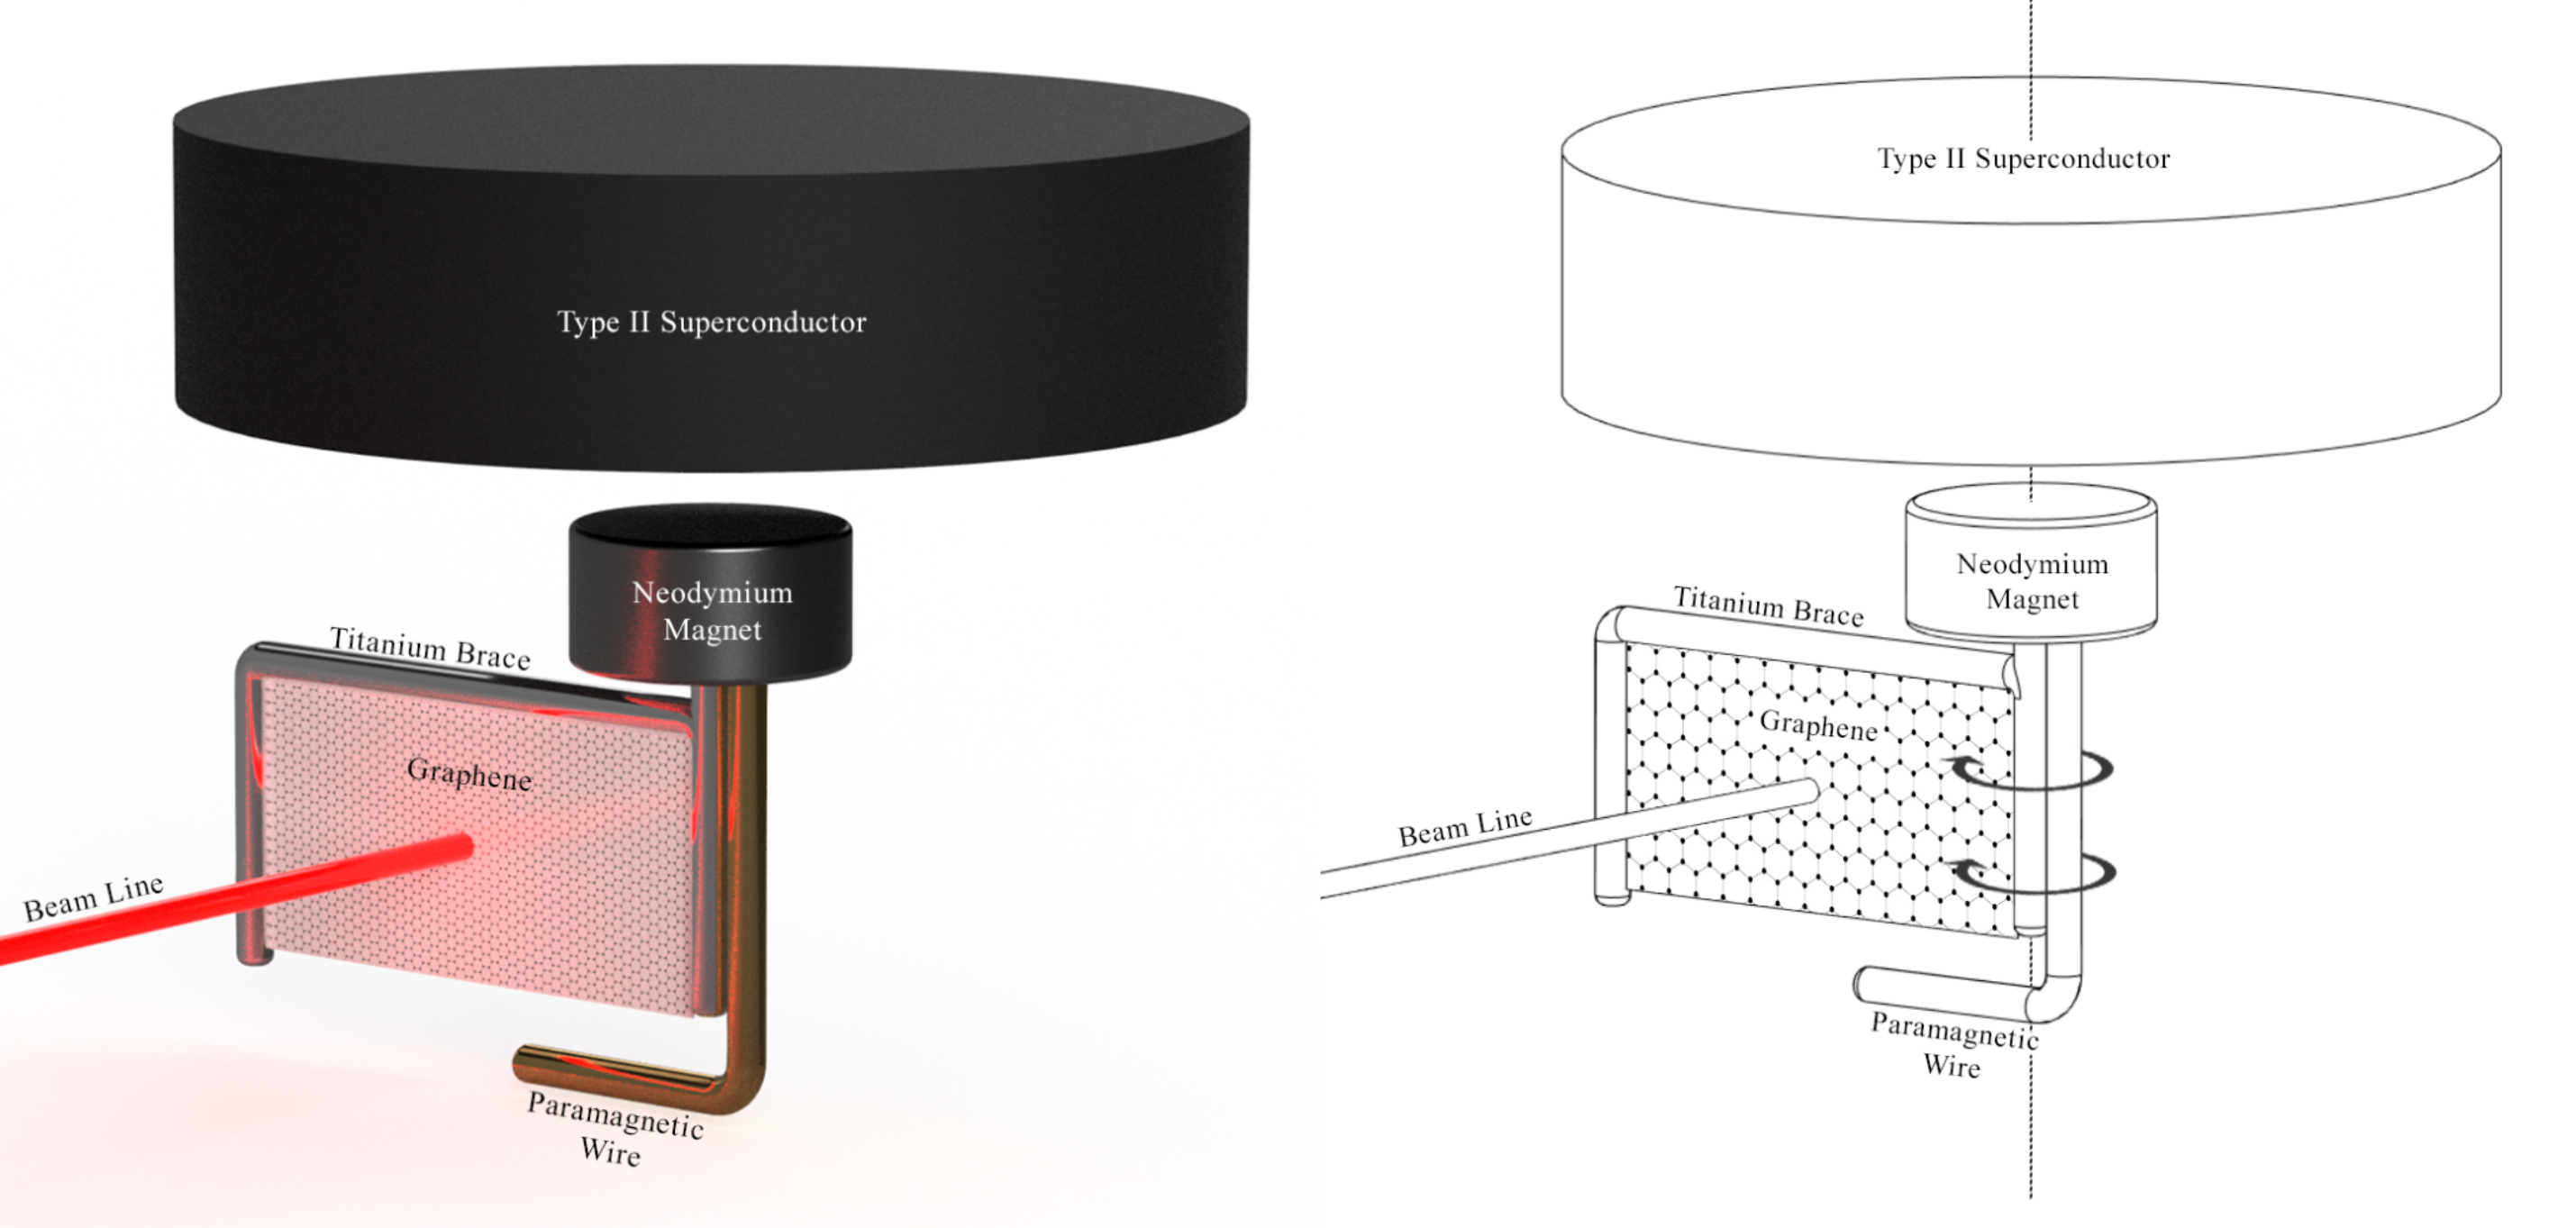
\includegraphics[scale=0.17]{color_monochrome_diagram.png}
    \caption{Color and monochromatic renderings of GRAPHS}
    \end{figure}

    \subsection{Calculations}

    \indent Inertias:
    \begin{itemize}
    \item Left titanium wire: $1.104\cdot10^{-14}\:\text{kg}\cdot\text{m}^2$
    \item Top titanium wire: $7.362\cdot10^{-15}\:\text{kg}\cdot\text{m}^2$
    \item Graphene: $1.267\cdot10^{-19}\:\text{kg}\cdot\text{m}^2$
    \item Neodymium magnet: $1.181\cdot10^{-14}\:\text{kg}\cdot\text{m}^2$
    \item Entire system: $3.021\cdot10^{-14}\:\text{kg}\cdot\text{m}^2$
    \end{itemize}

    \begin{enumerate}
    \item Momentum of a single particle, $p$, can be found through known values and particle speed
    \item Distance the particle will be from the center of rotation = $5\times10^{-4} \:\text{m}$
    \item Percentage of total particle momentum that goes into graphene rotation: $a$
    \item Angular momentum of the particle with respect to the center of rotation = $5p\cdot10^{-4}$
    \item Angular momentum of the graphene after the collision = $5ap\cdot10^{-4}$ ($0 < a \le 1$)
    \end{enumerate}

    $$L = I\omega$$
    $$5ap\cdot10^{-4}=3.021\cdot10^{-14}\cdot\omega$$
    $$\omega = 1.655\cdot10^{10}ap\: \text{rad/s}$$

    The particle beam shoots out $b$ photons per second, meaning that every second, the angular rotation speed of the graphene would increases by $1.655\cdot10^{10} abp$, giving an angular acceleration of $1.655\cdot10^{10}abp\: \frac{\text{rad}}{\text{s}^2}$

    $$\tau=I\alpha$$
    $$F_b\cdot5\cdot10^{-4}=3.021\cdot10^{14}\cdot1.655\cdot10^{10}abp$$
    $$F_b=abp\implies\text{Force exerted by }b\text{ particles.}$$
    $$\tau_b=5\cdot10^{-4}abp\implies\text{Torque caused by }b\text{ particles.}$$

For example, if we shoot a single proton with energy $25\text{GeV}$, its momentum would be roughly $1.33\cdot10^{-19}\:\frac{\text{kg}\cdot\text{m}}{\text{s}}$. Assuming an efficiency of $100\%$, the angular speed of the graphene would be $2.2\cdot10^{-9} \text{rad/s}$. With an increased number of particles, the hall effect sensor will be able to detect small changes. However, it is important to note that while, the particle number and efficiency has a linear relationship with force and torque, the moment of inertia has a more substantial effect due to the inverse square law.

\begin{figure}[H]
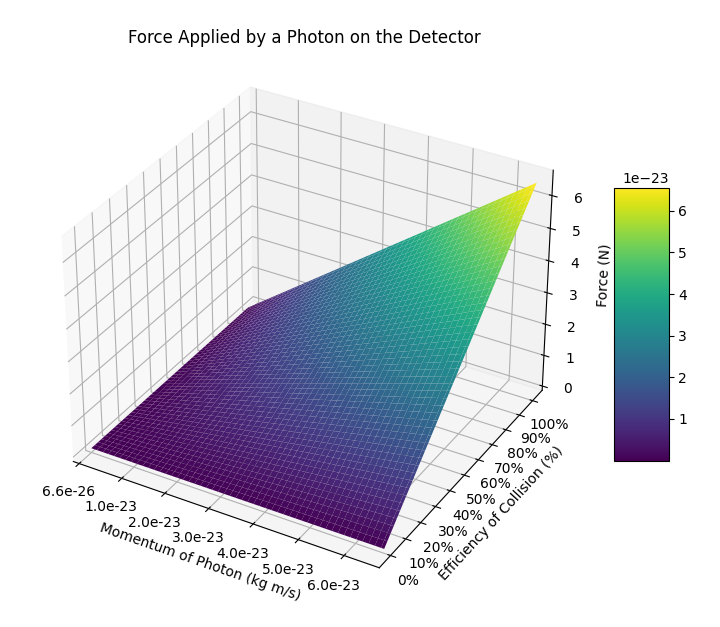
\includegraphics[scale=0.4]{force.png}
\caption{Force applied by a photon on the detector}
\end{figure}

\begin{figure}[H]
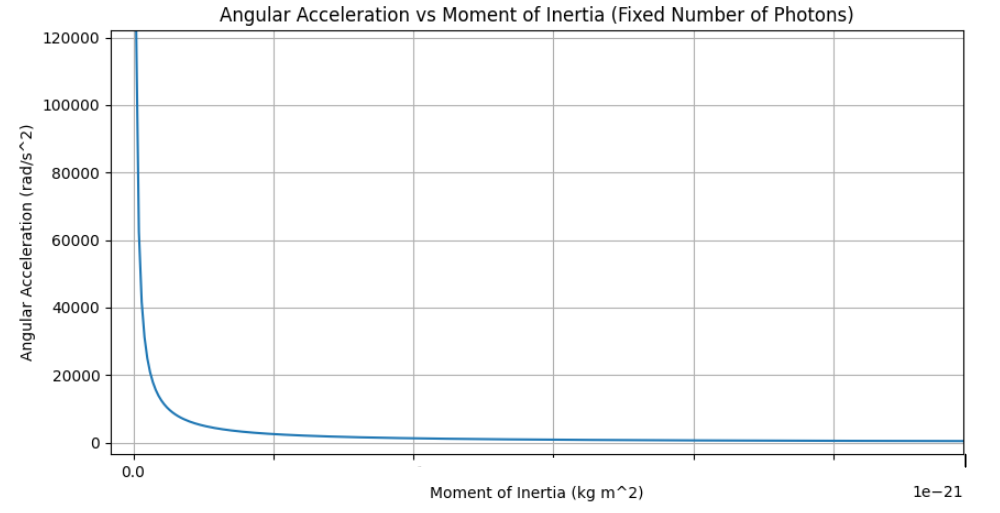
\includegraphics[scale=0.3]{acceleration.png}
\caption{Angular Acceleration vs. moment of inertia (fixed number of photons)}
\end{figure}

When shooting the particle beam, the values of $b$ and $p$ will be known while the value of $a$ will be experimentally determined.After gathering a value for $a$, it would be easier to estimate the force that a graphene solar-sail experiences due to particles striking it.

\subsection{Feasibility}

To set up experimental components, precise tools are necessary to dimension the graphene and assemble the small frame of the GRAPHS. We would need to caution for accidental mass that increases inertia, though our calculations show that the frame's inertia would be overcome by the particles' effect on the graphene. If the neodimyum is unsuitable for the beamline, the magnet type, as well as the wire frame type, could be altered with little change.

Inspired by the 2021 EXTRA team\cite{EXTRA}, we considered the possibility of a series of filters that would allow for a scattered xray to be detected by the GRAPHS, in the case that we cannot isolate protons through the use of our proposed setup. Using their Monte Carlo simulation, we have adjusted the heatmap to produce the relative torque values across the sensor, and due to the similar scale of the GRAPHS and the Mimosa sensors it would likely produce similar results.

\begin{figure}[H]
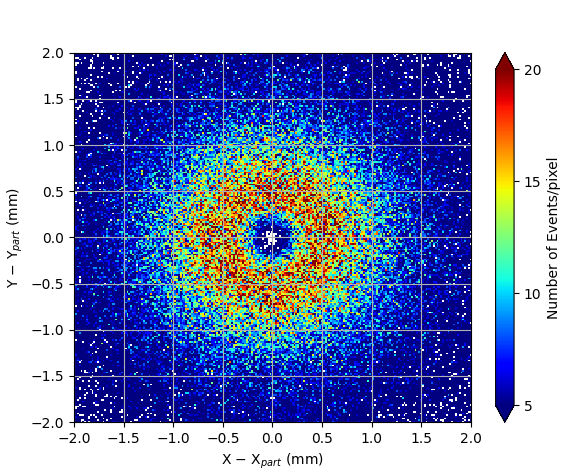
\includegraphics[scale=0.5]{extra.png}
\caption{EXTRA Team's Monte Carlo Positional Simulation}
\end{figure}

\begin{figure}[H]
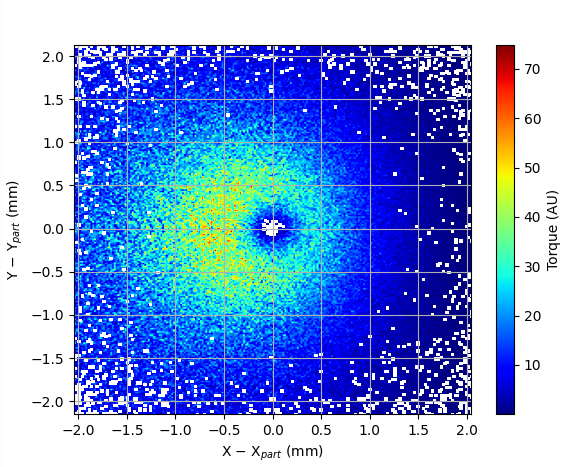
\includegraphics[scale=0.5]{our.png}
\caption{GRAPHS Team Adjusted for Relative Torque}
\end{figure}

    \subsection{Implications}

\indent A GRAPHS prototype would provide a mechanical alternative to other particle detectors. GRAPHS would output instant readings for the detection and energy of particles released into its path and will lend credibility to graphene's use in photon-powered solar sails.

\subsection{Additional Experiments}

\indent We have briefly considered other implications of graphenes properties, including a deformation based sensor for positional/energy data of single particles, and a capacative sensor that includes an array of Josephson junction sensors for photons.

\begin{figure}[H]
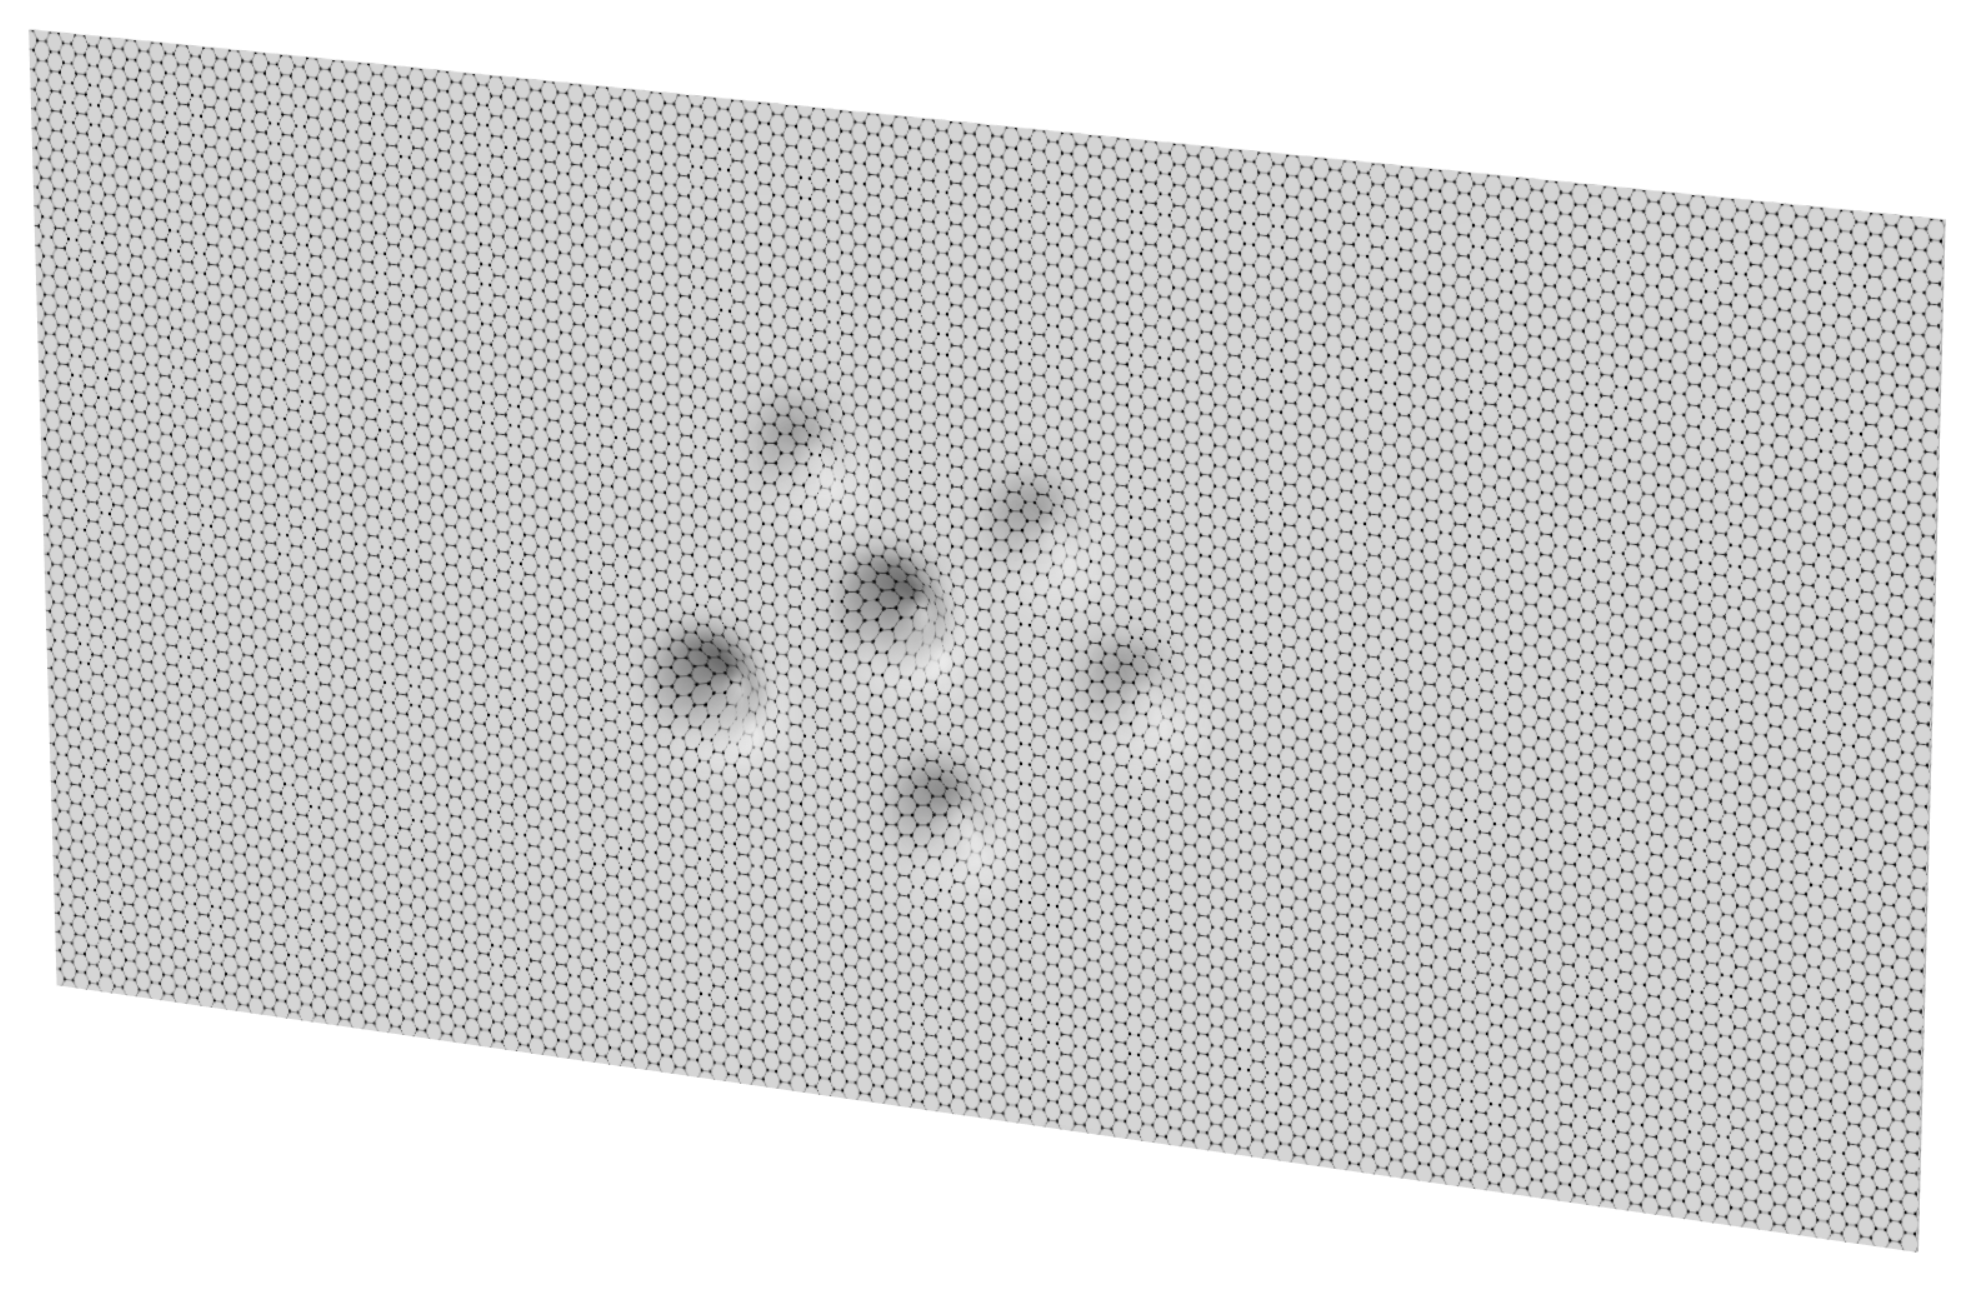
\includegraphics[scale=0.15]{deform.png}
\caption{Deformation to be sensed by piezoelectric sensors}
\end{figure}

\begin{figure}[H]
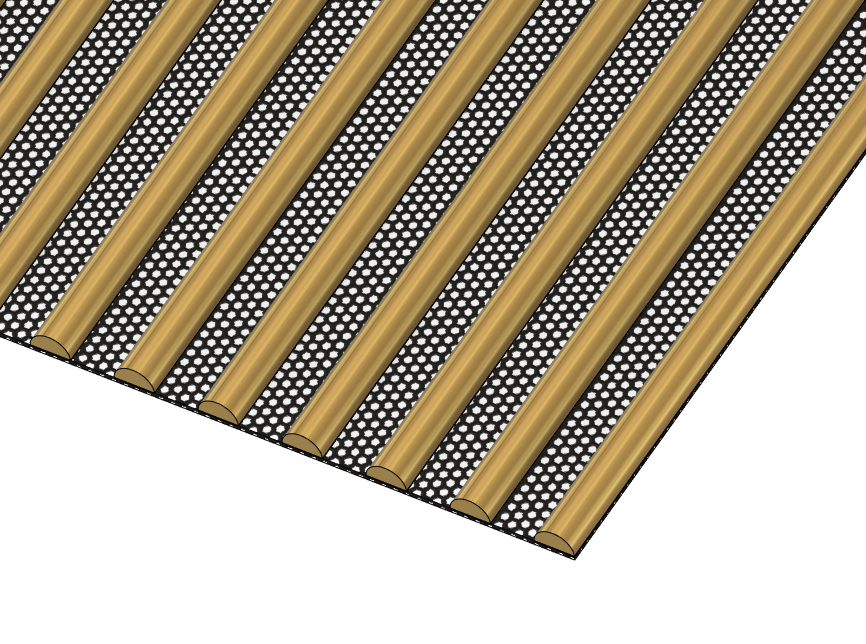
\includegraphics[scale=0.3]{junctions.png}
\caption{Render of 1D array of Josephson junctions}
\end{figure}

    \section{What we will take away from the experience}

    \indent Through research for our experiment alone, we have learned a great deal about particle physics. Experiencing the faculty and facilities at CERN would exponentially increase this knowledge while continuing our pursuits into physics. In terms of the research, we hope that our experiment will provide an alternative to other forms of detection while furthering interest in graphene. Regardless of our findings, we hope that this project will help inspire people within our high school and community to continue taking part in physics research, to increase interest within our generation and beyond.

    \section{Outreach}

    \indent We are all members of our school's modern physics club, which has exploded in popularity over the last few years. The hallmark of this club is that any passionate student is able to give presentations in any area of physics to the club. If we are able to conduct our experiment, we will be sure to present our experiences at CERN to people within our club and community. There are many in our school that are interested in scientific research, and we hope that this encourages students to pursue projects delving into science.

    \bibliographystyle{plain}
    \bibliography{beamline_for_schools.bib}
\end{document}